\bookchapter{บทที่ 37: ปฏิวัติกระบวนทัศน์ - จาก “เขียนโค้ด” สู่ “สั่งให้ AI เขียนโค้ด”}

\chapterintro{ยินดีด้วย คุณที่เปิดหนังสือเล่มนี้อยู่ตรงกลางของการปฏิวัติกระบวนทัศน์อาชีพพอดีเป๊ะ จุดเริ่มของการปฏิวัติครั้งนี้ คือประโยคหนึ่งที่โปรแกรมเมอร์คนหนึ่งโพสต์ลงโซเชียลมีเดียในปี 2025 ฟังดูดราม่าไปนิด? แต่ความจริงก็คืออย่างนั้น}

\booksection{กำเนิดของ Vibe Coding: ขบวนการที่เกิดจากประโยคเดียว}

กุมภาพันธ์ 2025 Andrej Karpathy - จดชื่อนี้ไว้ก่อน เดี๋ยวต้องเจอเขาอีกหลายครั้ง - โพสต์ทวีตขึ้นโซเชียลมีเดียที่ต่อมาถูกอ้างถึงไม่หยุด: “มีวิธีเขียนโปรแกรมแบบใหม่เรียกว่า Vibe Coding คือคุณให้เวท (vibes) นำจนหมด ละทิ้งรายละเอียดโค้ด ยกทุกอย่างให้ AI จัดการ เห็นอะไรก็บอกไป คัดลอกวาง ใช้ได้ก็โอเคแล้ว”

คำพูดที่ดูเหมือนโยนออกมาลอย ๆ นี้ จริง ๆ ตั้งชื่อให้การเปลี่ยนผ่านกระบวนทัศน์ที่เกิดขึ้นเงียบ ๆ แล้วอย่างแม่นยำ: มนุษย์ไม่ต้องเขียนโค้ดทีละบรรทัดอีกต่อไป แต่ใช้ภาษาธรรมชาติบรรยายความตั้งใจ แล้วให้ AI ทำส่วนที่เหลือ ถ้อยคำของ Karpathy มีกลิ่นล้อเลียนนิดหน่อย แต่ข้างหลังคือความเห็นที่ลึกซึ้ง: เมื่อความสามารถสร้างโค้ดของ AI ก้าวข้ามเส้นบางเส้นไปแล้ว คอขวดของการเขียนโปรแกรมไม่ใช่ “บรรทัดนี้ฉันเขียนออกไหม” อีกต่อไป แต่เป็น “เรื่องนี้ฉันคิดชัดจริงหรือเปล่า”

\begin{tcbinfo}{เคล็ดลับเล็ก ๆ: Vibe คืออะไร?}
Vibe แปลตรงตัวคือ “บรรยากาศ ความรู้สึก” Vibe Coding ก็คือ “คุม AI เขียนโปรแกรมโดยให้ความรู้สึกนำ” คุณบรรยายว่าอยากได้อะไร AI จัดการทำให้ จดคำนี้ไว้ เพราะมันคือ “ใบเกิด” ของการปฏิวัติครั้งนี้

\end{tcbinfo}

นับจากวินาทีนั้น ความหมายของคำว่า “โค้ดดิ้ง” เริ่มแยกออกจากกัน: โค้ดดิ้งแบบเดิมคือการแปลดีไซน์เป็นไวยากรณ์ ส่วนโค้ดดิ้งแบบใหม่คือการแปลความตั้งใจเป็นคำสั่ง อย่างแรกทดสอบนิ้ว อย่างหลังทดสอบสมอง

คำว่า Vibe Coding เปลี่ยนจากเรื่องล้อเลียนเป็นมโนทัศน์ทางวิศวกรรมจริงจังอย่างรวดเร็ว มาถึงกลางปี 2026 มันได้วิวัฒน์จากมีมบนโซเชียล กลายเป็นระบบวิธีการที่สมบูรณ์ ครอบคลุมกระบวนการเต็มตั้งแต่การสื่อสารความต้องการ การจัดการบริบท การตรวจสอบแบบทำซ้ำ ไปจนถึงการการันตีคุณภาพ ผู้คนยังตระหนักว่า “ตามความรู้สึก” เป็นแค่สภาพของช่วงเริ่มต้น การเขียนโปรแกรมด้วย AI ที่มีประสิทธิภาพจริงต้องใช้แนวคิดแบบเป็นระบบ และแนวคิดแบบนั้น ก็คือสิ่งที่หนังสือเล่มนี้จะมอบให้คุณ

\booksection{สถานการณ์ปี 2026: ยุคของ Agentic Engineering}

มาถึงสิงหาคม 2026 วงการเขียนโปรแกรมด้วย AI ผ่านการยกระดับกระบวนทัศน์มาหลายรอบแล้ว Vibe Coding คือประกายไฟเริ่มต้น แต่ทุกคนก็พบเร็ว ๆ ว่า: แค่แชทกับ AI แบบ “ตามความรู้สึก” ล้วน ๆ คุณภาพโค้ดที่ได้ไม่นิ่งเลย ครั้งหนึ่งก็ว้าว ครั้งหนึ่งก็พัง กระบวนทัศน์จึงเริ่มวิวัฒน์ จากการเขียนโปรแกรมแบบคุยโต้ตอบง่าย ๆ ไปสู่วิศวกรรม Agent ที่มีโครงสร้าง

และก็เป็น Karpathy อีกนั่นแหละ ต้นปี 2026 เขาเสนอมโนทัศน์ Agentic Engineering ต่างจาก Vibe Coding ที่ “พูดแล้วสร้าง” ตรงที่ Agentic Engineering เน้นว่า: ให้เป้าหมายแก่ AI แล้วปล่อยให้มันวางแผนขั้นตอน เรียกใช้เครื่องมือ ตรวจสอบผลลัพธ์ และแก้ไขเป็นรอบ ๆ ด้วยตัวเอง AI ไม่ใช่แค่เครื่องสร้างโค้ดอีกต่อไป แต่เป็นเอเจนต์ (Agent) ที่รับรู้สภาพแวดล้อม ตัดสินใจ และลงมือทำได้

การเปลี่ยนผ่านนี้นำมาซึ่งการเปลี่ยนแปลงสำคัญสามประการ:

\begin{enumerate}
  \item รูปแบบการโต้ตอบเปลี่ยน: จาก "ถามทีตอบที" เป็น "ตั้งเป้าหมายแล้วมอบอำนาจ"
  \item ผลงานที่ได้เปลี่ยน: จาก "โค้ดหนึ่งชุด" เป็น "โปรเจกต์ที่สมบูรณ์หนึ่งชิ้น"
  \item บทบาทของคนเปลี่ยน: จาก "ตรวจโค้ดทีละบรรทัด" เป็น "กำหนดขอบเขตและตรวจรับผลลัพธ์"
\end{enumerate}

ตัวเลขไม่เคยโกหก: ใน Cursor 3 ที่ปล่อยเมษายน 2026 อัตราการใช้โหมด Agent แซงโหมด Tab completion ไปได้เป็นครั้งแรก ซึ่งบอกว่านักพัฒนาได้ย้ายมาใช้วิธีทำงานแบบนี้กันเป็นวงกว้างแล้ว ส่วน Claude Code ซึ่งเป็นเครื่องมือเขียนโปรแกรมด้วย AI ที่อยู่บนเทอร์มินัลโดยตรง มาถึงกลางปี 2026 รายได้ที่คิดเป็นรายปีทะลุ 2.5 พันล้านดอลลาร์ไปแล้ว กราฟแนวโน้มข้างล่างจะให้คุณสัมผัสช่วงเวลาตัดกันตรงนี้ได้แบบเห็นภาพ:

\begin{center}
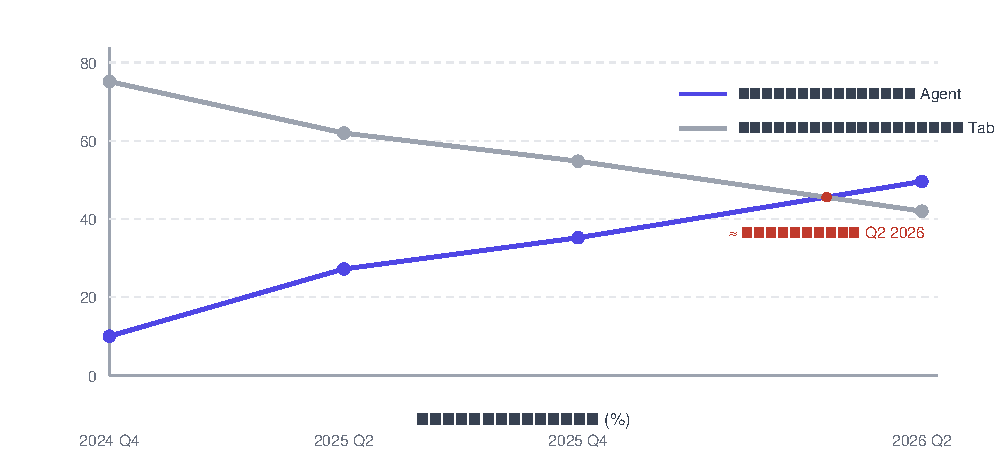
\includegraphics[width=0.92\linewidth]{figures/fig-di-san-shi-qi-zhang-1}
\\[2pt]\small ภาพที่ 1: แนวโน้มอัตราการใช้โหมดโต้ตอบของ AI ในการเขียนโปรแกรม (ประมาณการจากข้อมูลสำรวจอุตสาหกรรม ไตรมาส 2/2026 โหมด Agent แซง Tab completion)
\end{center}

แต่พูดกันตรง ๆ: การเปลี่ยนของเครื่องมือและโมเดลเป็นแค่ผิวนอก ไม่ว่าคุณจะใช้ Cursor หรือ Claude Code ไม่ว่าโมเดลรากฐานจะเป็น GPT-5 หรือ Claude 4.5 คนที่ประสบความสำเร็จกับการเขียนโปรแกรมด้วย AI ล้วนยึดวิธีการพื้นฐานชุดเดียวกัน และนี่คือสิ่งที่คู่มือนี้จะสอนคุณ

\booksection{การเปลี่ยนแปลงความคิดแกนกลาง: จาก Coder สู่ Conductor}

การศึกษาเขียนโปรแกรมแบบเดิมสอนให้คุณเป็น Coder - เข้าใจไวยากรณ์ จำ API ดีบักข้อผิดพลาดตรรกะ แต่ยุคการเขียนโปรแกรมด้วย AI บทบาทนี้กำลังถูกนิยามใหม่ คุณไม่ต้องเขียนโค้ดทุกบรรทัดด้วยมือเองอีกต่อไป แต่คุณต้องกลายเป็น “ผู้อำนวยเพลง” (Conductor): กำหนดสมรภูมิ วางกฎเกณฑ์ แบ่งงาน และตรวจรับผลงาน

แกนของการเปลี่ยนผ่านนี้ไม่ได้อยู่ที่ “คุณเขียนโค้ดเป็นไหม” แต่อยู่ที่ “คุณคิดชัดไหมว่าจะทำอะไร” ผู้บัญชาการที่เก่งไม่จำเป็นต้องเป็นทหารที่ดีที่สุด แต่เขาต้องเข้าใจเป้าหมายของยุทธการ ภูมิประเทศ และการจัดกำลังได้ดีที่สุด ในทำนองเดียวกัน คนที่เก่งเรื่องเขียนโปรแกรมด้วย AI ไม่จำเป็นต้องชำนาญไวยากรณ์ของทุกภาษา แต่เขาต้องชัดที่สุดกับเป้าหมายโปรเจกต์ ข้อจำกัดของสถาปัตยกรรม และมาตรฐานคุณภาพ

ตารางนี้คุ้มค่าที่จะอ่านซ้ำอีกสองรอบ เพราะมันสรุปแก่นทั้งหมดของการเปลี่ยนบทบาทครั้งนี้ไว้:

\begin{center}
\begin{tabularx}{\linewidth}{|X|X|X|}
\hline
\textbf{มิติ} & \textbf{Coder แบบดั้งเดิม} & \textbf{ผู้อำนวยเพลง AI (Conductor)} \tabularnewline
\hline
ทักษะหลัก & จำไวยากรณ์ เรียก API ดีบัก & นิยามความต้องการ จัดการบริบท วิเคราะห์การตรวจรับ \tabularnewline
วิธีทำงาน & เขียนโค้ดทีละบรรทัด & บรรยายความตั้งใจ ตรวจทานผลงาน \tabularnewline
การควบคุมคุณภาพ & เขียนเองก็รู้ในใจว่าเป็นอย่างไร & ยืนยันผลงาน AI ผ่านการทดสอบและการตรวจสอบ \tabularnewline
ความรู้ที่ต้องใช้ & เชี่ยวชาญลึกในภาษา/เฟรมเวิร์กเฉพาะตัว & เข้าใจภาพรวมเทคโนโลยีกว้าง เข้าใจตรรกะธุรกิจลึก \tabularnewline
คอขวดอยู่ที่ไหน & ความเร็วในการเขียนโค้ดและการจำไวยากรณ์ & ความชัดเจนในการคิดและความสามารถสื่อสาร \tabularnewline
แหล่งที่มาของข้อผิดพลาด & ไวยากรณ์ผิด ตรรกะตกหล่น & ความต้องการคลุมเครือ บริบทไม่พอ \tabularnewline
\hline
\end{tabularx}
\end{center}

\begin{center}\small\color{gray}เปรียบเทียบมิติความสามารถระหว่าง Coder แบบดั้งเดิมกับผู้อำนวยเพลง AI\end{center}

นี่ไม่ได้แปลว่าความรู้การเขียนโปรแกรมไม่สำคัญแล้วหรอกนะ กลับกันเลย: ก็ต่อเมื่อคุณอ่านโค้ดที่ AI เขียนออกได้ คุณถึงจะตรวจสอบและแก้ไขมันได้อย่างมีประสิทธิภาพ ก็ต่อเมื่อคุณเข้าใจโครงสร้างข้อมูลและอัลกอริทึม คุณถึงจะตัดสินได้ว่าแนวทางที่ AI เสนอสมเหตุสมผลไหม คลังความรู้กำหนด “เพดานการอำนวยการ” ของคุณ แต่บทบาทของความรู้เปลี่ยนจาก “เครื่องมือลงมือทำ” มาเป็น “หลักยึดในการตัดสินใจ”

\booksection{ทำไมวิธีคิดจึงสำคัญกว่าเครื่องมือ}

เครื่องมือปรับใหม่ทุกสามเดือน แต่วิธีการพัฒนาทุกสามปี ใช้เครื่องมือเก่งอาจล้าสมัยในสามเดือน แต่มีวิธีคิดที่ดียังใช้ได้อีกสามปี

หลายคนพอเริ่มเขียนโปรแกรมด้วย AI สิ่งแรกที่ถามคือ “เครื่องมือไหนดีที่สุด” “โมเดลไหนแกร่งสุด” คำถามพวกนี้ไม่ได้ไม่สำคัญ แต่ถามลำดับความสำคัญผิดไป ภูมิทัศน์เครื่องมือเดือนสิงหาคม 2026 ต่างจากสิงหาคม 2025 สุดขั้วแล้ว - เครื่องมืออย่าง Trae, Qoder ขึ้นแล้วก็ลง, Cursor เปลี่ยนจากปลั๊กอินเป็น IDE แยกต่างหากแล้วไต่ไปถึง Cursor 3, Claude Code จากโปรเจกต์ทดลองกลายเป็นทางเลือกหลักของการเขียนโปรแกรมบนเทอร์มินัล แต่หลังการเปลี่ยนแปลงรุนแรงนี้ หลักคิดที่คนสำเร็จยึดถือแทบไม่เปลี่ยนเลย

นี่คือเหตุผลที่หนังสือเล่มนี้จะไม่เสียพื้นที่ไปสอนวิธีใช้เครื่องมือตัวใดตัวหนึ่งเป็นรูปเป็นร่าง - พอเขียนจบก็ล้าสมัยทันที ตรงกันข้าม หนังสือเล่มนี้วางน้ำหนักทั้งหมดไว้ที่วิธีคิดหนึ่งชุดที่ผ่านการพิสูจน์แล้ว: คิดถึงความต้องการอย่างไร สื่อสารกับ AI อย่างไร ตรวจยอมผลงานอย่างไร ทำซ้ำต่อเนื่องอย่างไร พอเชี่ยวชาญวิธีคิดชุดนี้ คุณเปลี่ยนไปใช้เครื่องมือไหนก็เข้าที่เร็ว แต่ถ้าได้แค่วิธีกดปุ่ม พอเปลี่ยนเครื่องมือก็ต้องเริ่มนับหนึ่งใหม่

\begin{tcbinfo}{ยาใจสำหรับผู้อ่านที่เริ่มจากศูนย์}
ถ้าคุณเริ่มจากศูนย์ อย่าโดนคำว่า “วิธีการ (methodology)” ข่มขู่ วิธีการไม่ใช่ปรัชญานามธรรม มันคือคู่มือปฏิบัติหนึ่งชุดเรื่อง “เจอปัญหาแล้วควรคิดยังไง” เหมือนเวลาเรียนทำอาหาร: คุณทำตามสูตรทีละขั้นได้ (วิธีใช้เครื่องมือ) แต่เชฟมืออาชีพเข้าใจคือ “ทำไมต้องปรุงแบบนี้” “คุมไฟอย่างไร” (วิธีการ) หนังสือเล่มนี้จะเริ่มจากมโนทัศน์พื้นฐานที่สุด ทุกหลักการมาพร้อมกรณีเปรียบเทียบที่เป็นรูปธรรม เพื่อให้คุณไม่ใช่แค่เข้าใจ “คืออะไร” แต่คว้า “ทำอย่างไร” ไว้ได้ด้วย

\end{tcbinfo}

\begin{tcbpractice}{มาลงมือ: ถ่าย "ภาพบทบาท" ของคุณในตอนนี้}
เอากระดาษมาแผ่น จดคำตอบของสามคำถามนี้: (1) ตอนนี้คุณใช้ AI ช่วยเขียนโค้ดอย่างไร (ถ้าเคยใช้)? (2) คุณเหมือน “Coder” ในตารางข้างบนหรือ “ผู้อำนวยเพลง” มากกว่า? (3) คุณอยากให้ตัวเองในอีกสามเดือนบรรยายวิธีทำงานของตัวเองว่าอย่างไร? เขียนเสร็จแล้วแหน่ไว้ในหนังสือ อ่านจบบทที่ 47 แล้วกลับมาดูอีกที คุณจะพบว่าการเปลี่ยนแปลงเร็วกว่าที่คิด

\end{tcbpractice}

\begin{tcbsummary}{สรุปบทนี้}
\begin{itemize}
  \item ปี 2025 Karpathy ตั้งชื่อการปฏิวัติการเขียนโปรแกรมด้วย AI ว่า "Vibe Coding": จากการเขียนโค้ดทีละบรรทัด มาเป็นการบรรยายความตั้งใจด้วยภาษาธรรมชาติ
  \item ปี 2026 วิวัฒน์สู่ Agentic Engineering: ให้เป้าหมาย มอบอำนาจ AI วางแผนลงมือเอง คนรับผิดชอบการตรวจรับ
  \item อัตราใช้โหมด Agent ของ Cursor 3 แซง Tab completion เป็นครั้งแรก; รายได้รายปีของ Claude Code แตะ 2.5 พันล้านดอลลาร์
  \item บทบาทใหม่ของคุณคือ Conductor (ผู้อำนวยเพลง): กำหนดสมรภูมิ วางกฎ แบ่งงาน ตรวจรับผลงาน
  \item เครื่องมือหมุนเวอร์ชันทุกสามเดือน วิธีการพัฒนาทุกสามปีเท่านั้น - เรียนวิธีการ ไม่ใช่วิธีกดปุ่ม
\end{itemize}

\end{tcbsummary}
